\chapter{Introduction}
\section{Biological background}
Systems biology is a multidisciplinary field, drawing from biology, mathematics, and computer science. In this section, I first provide a background on the biology of circadian rhythms, followed by previous literature on computational modeling. 

Ecological competition drives species to optimize their survival and reproduction in a particular environmental niche. Aspects of their environment, including temperature, resource availability, and sunlight are all important factors in determining an individual's success.

In nearly all environments, however, these factors vary greatly from hour to hour and month to month. While food or sunlight might be plentiful during daylight hours, the threat of predators might peak as well. Fortunately, while these critical parameters undergo sharp changes, they do so with a predictable and repeatable schedule. It is not surprising that, in optimizing their survival in an oscillating environment, species have developed a means to predict changes and to ready themselves for the correct behavior.

Biological rhythms are classified as {\em circadian} if they display a number of defining characteristics:
\begin{itemize}
  \item They are {\em endogenous}, meaning they continue to oscillate even when the organism is isolated from its environment

  \item They are temperature compensated, maintaining a consistent period for moderate changes in average temperature

  \item They are {\em entrainable}, meaning they can adjust their phase and period in response to a changing in environmental signal

  \item They oscillate with a roughly 24 hour period \cite{Dunlap2009}.

\end{itemize}

\begin{figure}
  \centering
  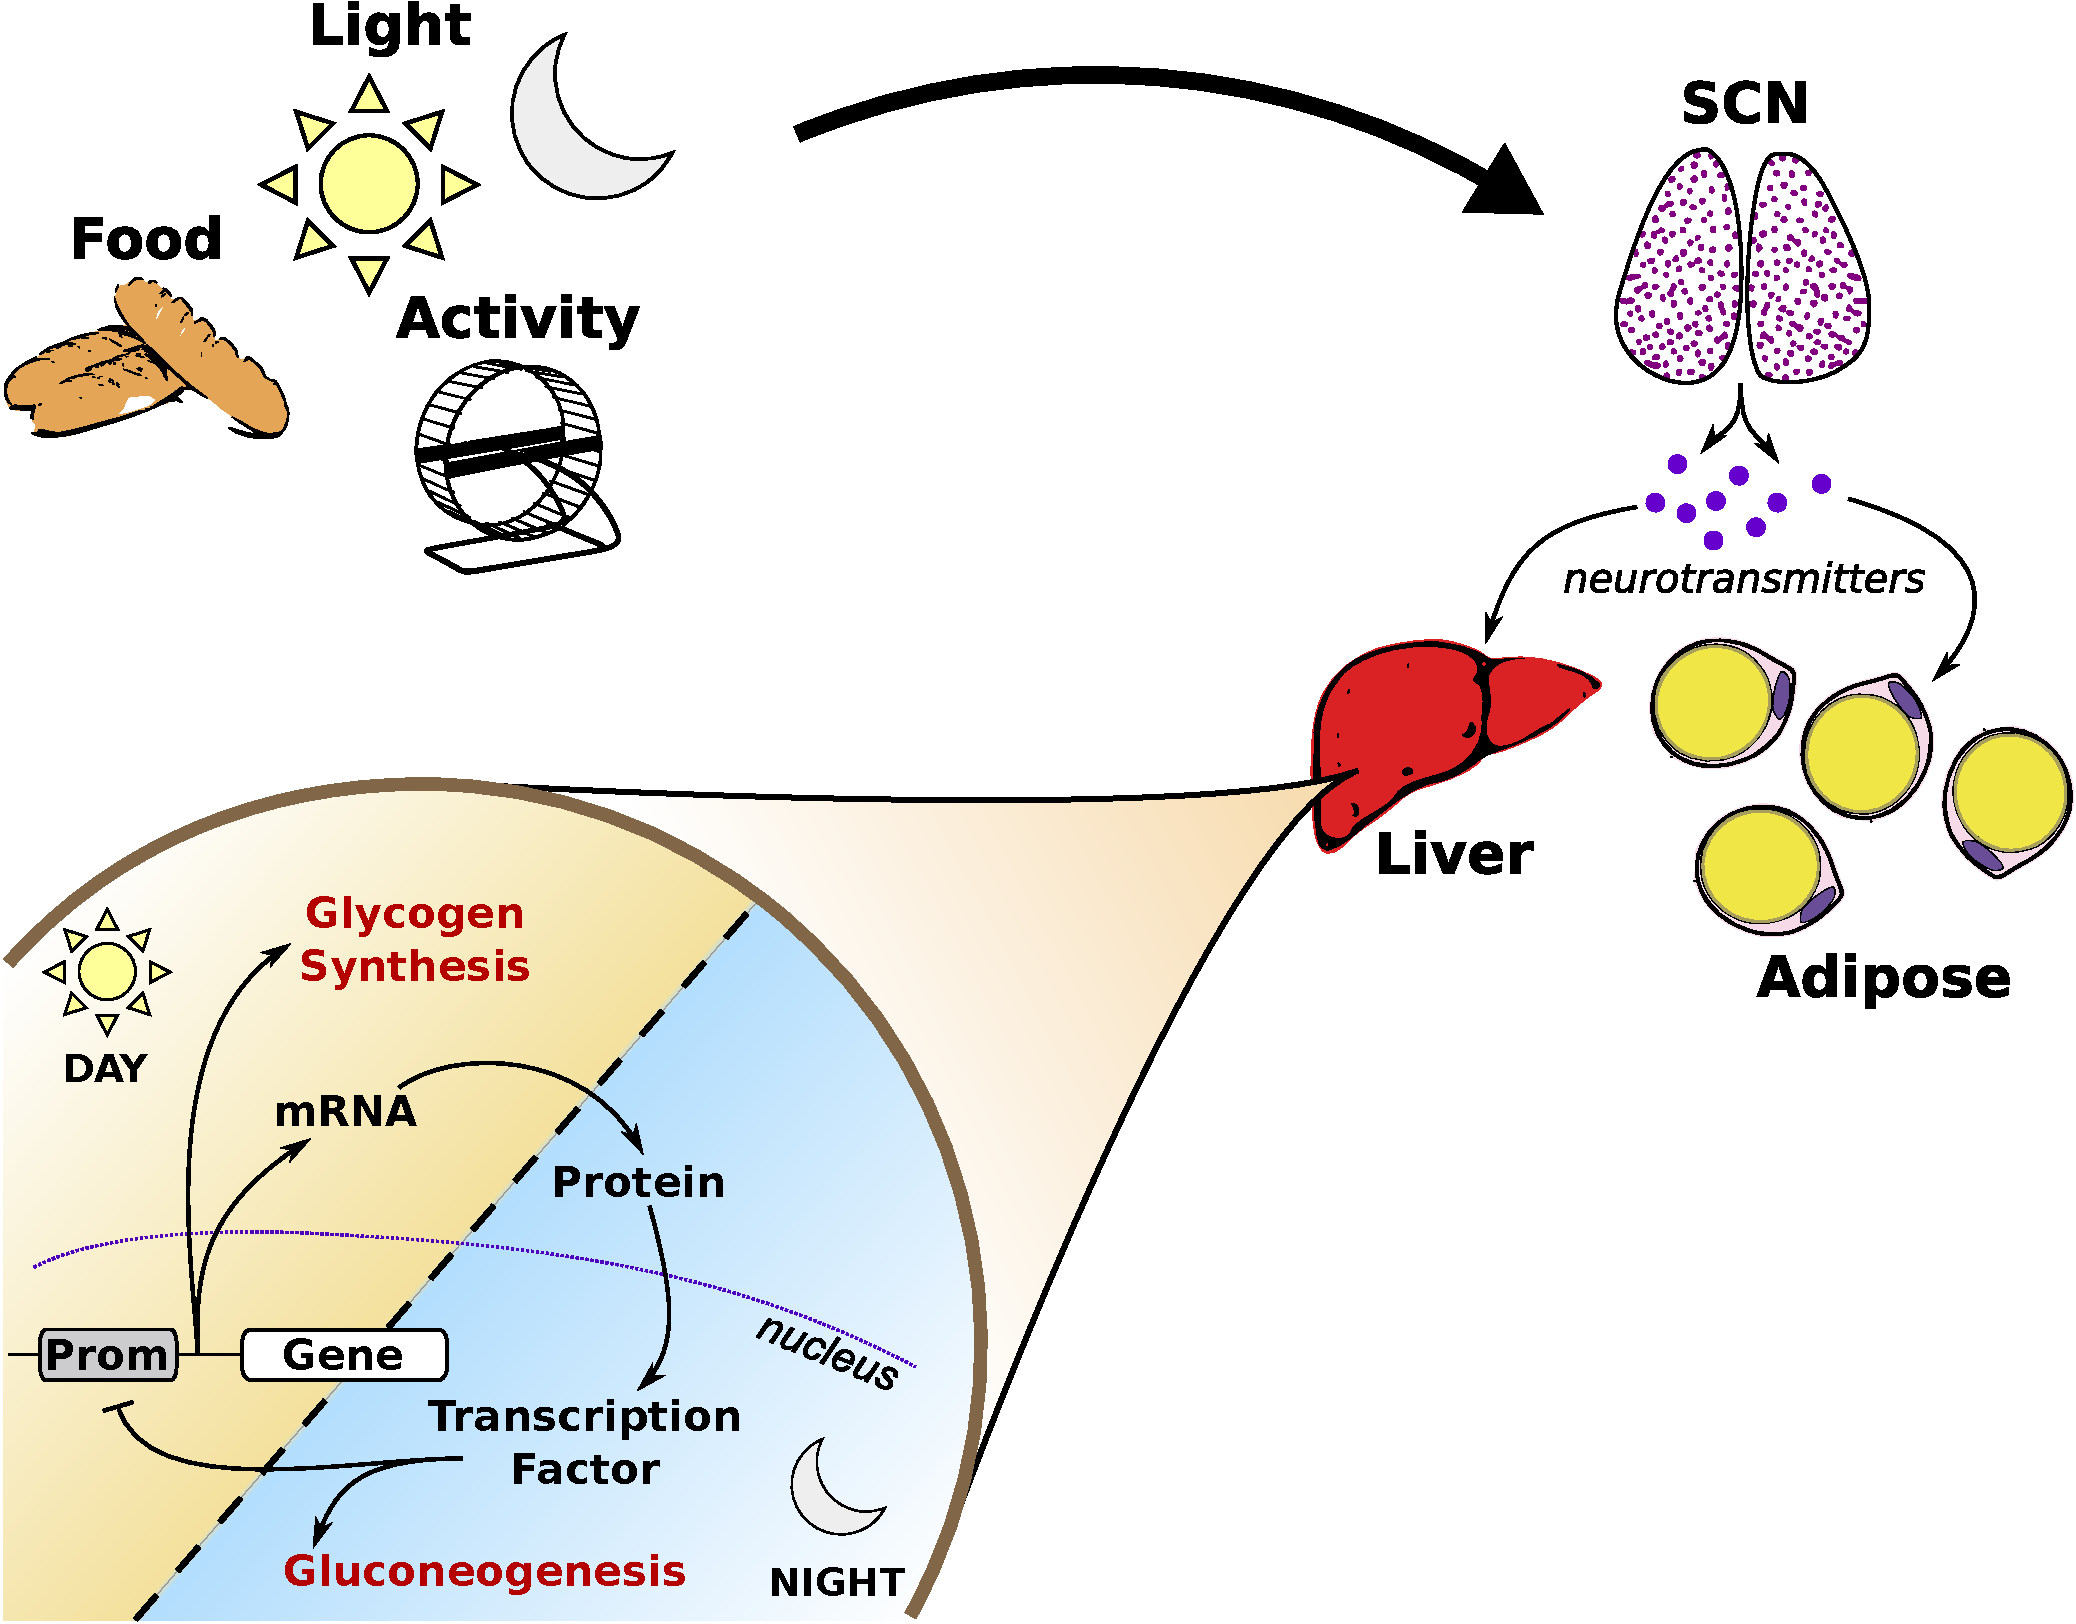
\includegraphics[width=\textwidth]{chap1/figures/timescale_separation.pdf}
  \titlecaption{A biological feed forward controller}{Circadian rhythms}
  \label{fig:feedforward}
\end{figure}

\subsection{Evolutionary history}\blindtext
\subsection{Mechanisms of gene regulation}\blindtext
\subsection{Mammalian genetic circuit}\blindtext
\section{Mathematical modeling}\blindtext
\subsection{Overview of kinetic ODE models}\blindtext
\subsubsection{Spectrum of modeling methods (detail vs. scope)}\blindtext
\subsection{Basic terms and assumptions}\blindtext
\subsubsection{Mass action}\blindtext
\subsubsection{Michealis-Menten}\blindtext
\subsubsection{Hill-type}\blindtext
\subsection{Simulation methods}\blindtext
\subsubsection{Numerical solution of nonlinear ODEs}\blindtext
\subsubsection{Boundary value problem for limit cycle models}\blindtext
\subsection{ODE Sensitivity Analysis}\blindtext
\subsubsection{ODEs in general}\blindtext
\subsubsection{Period sensitivity}\blindtext
\subsubsection{PRCs}\blindtext
\subsection{Previous models of circadian rhythms}\blindtext
